\documentclass[11pt]{article}
\usepackage[utf8]{inputenc}
\usepackage[T1]{fontenc}
\usepackage{amsmath,amssymb}
\usepackage{booktabs}
\usepackage{graphicx}
\usepackage{geometry}
\geometry{margin=1in}
\usepackage{authblk}
\usepackage[hidelinks]{hyperref}
\usepackage{caption}


\title{\textbf{Explainable Credit Default Prediction for Microfinance:\\
A Gradient Boosting and SHAP Study on Consumer Credit Data}}

\author[1]{Craig Carlos Ouma\thanks{%
Correspondence: \texttt{craigcarlos95@gmail.com}}}
\affil[1]{Independent Researcher}
\date{\today}

\begin{document}
\maketitle

\begin{abstract}
\noindent
Credit scoring models underpin lending decisions for millions of borrowers, yet in many
microfinance settings they operate as black boxes --- lenders know the score but not the
story behind it. This paper trains and compares three classifiers (Logistic Regression,
XGBoost, and LightGBM) on the Give Me Some Credit consumer credit dataset (150,000
borrowers, 6.68\,\% default rate) and applies SHAP (SHapley Additive exPlanations)
to make the best-performing model's decisions transparent. All three classifiers perform
within a narrow AUROC band of 0.862--0.868, with XGBoost leading marginally
(AUROC\,=\,0.868, Gini\,=\,0.735, KS\,=\,0.581). The SHAP analysis reveals that two
features --- revolving credit utilisation and maximum delinquency status ---
together drive the bulk of predictive signal, a finding consistent with established
credit theory. Younger borrowers and those with lower incomes face systematically
higher predicted default risk, while the effect of revolving utilisation is
notably non-linear: risk rises sharply once utilisation crosses 0.5. We also find
that all three tree models are poorly calibrated, meaning raw predicted probabilities
should not be used directly as default rates without recalibration. These results
suggest that gradient boosting combined with SHAP offers a practical and explainable
credit scoring framework for microfinance lenders who need both predictive accuracy
and regulatory transparency.
\end{abstract}

\section{Introduction}

Credit scoring has a long history, but the way it gets done in practice has changed
considerably. Traditional scorecards were linear, interpretable by design, and easy
to audit --- a loan officer could understand why a borrower scored the way they did.
Modern machine learning models are more powerful, but that power usually comes with
opacity. For a microfinance institution in East Africa, this creates a real problem:
regulators increasingly require that lending decisions be explainable, and borrowers
have a right to understand why they were declined~\cite{barocas2023fairness}.

The dominant approach to bridging this gap is SHAP, introduced by Lundberg and
Lee~\cite{lundberg2017shap}. SHAP provides each feature with a contribution score
for each individual prediction, grounded in cooperative game theory. Unlike simpler
importance measures (gain, split count), SHAP values have a rigorous theoretical
basis and can be aggregated across borrowers to give a population-level picture of
what drives default risk. This makes them useful not just for debugging models but
for regulatory disclosure and for training loan officers.

We apply this framework to the Give Me Some Credit dataset, which provides a realistic
snapshot of US consumer credit behaviour. While the data originates from the US, the
modelling problem --- predicting serious delinquency from payment history,
income, and credit utilisation --- is structurally identical to what microfinance
lenders face in markets like Kenya, where mobile credit products have created large
portfolios of thin-file borrowers with limited formal credit history.

Our goals are modest and practical: train well-tuned classifiers, compare them honestly
using metrics that credit teams actually care about (Gini coefficient and KS statistic,
not just AUROC), and then use SHAP to understand what the best model has learned.

\section{Related Work}

\textbf{Credit scoring with machine learning.} Gradient boosting methods have
consistently outperformed logistic regression on credit datasets in the
literature~\cite{lessmann2015benchmarking}, and XGBoost in particular has dominated
credit-related Kaggle competitions since its
introduction~\cite{chen2016xgboost}. LightGBM offers comparable performance
with faster training, making it attractive for deployment on constrained
infrastructure~\cite{ke2017lightgbm}.

\noindent\textbf{Explainability in credit models.} SHAP has become the dominant
interpretability tool for tabular credit models, partly because it satisfies
desirable axioms (efficiency, symmetry, dummy, and additivity) that simpler
feature importance measures do not~\cite{lundberg2017shap}. Several recent studies
have applied SHAP to credit default datasets and found that revolving
utilisation and payment history consistently dominate feature importance
rankings~\cite{bussmann2021explainability}, a finding we replicate here.

\noindent\textbf{Microfinance and alternative credit scoring.}
Traditional credit bureau data is unavailable for a large share of borrowers in
sub-Saharan Africa. Research on alternative data sources --- mobile money
transactions, utility payments, psychometric testing --- is active, but the
modelling methodology developed on traditional datasets transfers
directly~\cite{demirguc2018financial}.

\section{Data}

The Give Me Some Credit dataset was originally released as a Kaggle competition
by TransUnion in 2011. It contains 150,000 labelled observations of US consumer
borrowers, each described by ten features drawn from credit bureau records.
The prediction target is \texttt{SeriousDlqin2yrs}: whether the borrower
experienced a delinquency of 90 or more days past due within the following
two years.

\paragraph{Class imbalance.} The dataset is imbalanced: 10,026 borrowers (6.68\,\%)
defaulted and 139,974 (93.32\,\%) did not. This is realistic --- most credit
portfolios have single-digit default rates --- but it means naive classifiers
that predict no default on every borrower would achieve 93.3\,\% accuracy
while being completely useless.

\paragraph{Missing data.} Two features have substantial missingness:
\texttt{MonthlyIncome} (19.8\,\% missing) and \texttt{NumberOfDependents}
(2.6\,\% missing). Both were imputed using column medians. Importantly,
missingness in income is not random --- borrowers without reported income
are systematically different, which we flag as a limitation.

\paragraph{Data quality issues.} The three delinquency count columns
(\texttt{NumberOfTime30-59DaysPastDueNotWorse},
\texttt{NumberOfTimes90DaysLate},
\texttt{NumberOfTime60-89DaysPastDueNotWorse}) contain values of 96 and 98
that appear to be sentinel codes for unknown or erroneous data rather than
genuine counts. These were replaced with \texttt{NaN} and the columns were
subsequently capped at 10 to prevent extreme values from dominating splits.
\texttt{RevolvingUtilizationOfUnsecuredLines} had values up to 50,708 despite
being defined as a ratio between 0 and 1; these were capped at 1.0. One
borrower with \texttt{age}\,=\,0 was treated as invalid and imputed.

\paragraph{Feature engineering.} Six derived features were constructed:
\texttt{MaxDelqStatus} (maximum across the three delinquency columns),
\texttt{TotalDelinquencies} (sum), \texttt{AnyDelinquency} (binary indicator),
\texttt{MonthlyIncome\_log} (log-transformed income),
\texttt{IncomePerDependent} (income divided by dependents plus one),
and \texttt{EstMonthlyDebt} (debt ratio times income, approximating
monthly debt burden). The final feature set contains 16 predictors.

\section{Methods}

\subsection{Models}

We train three classifiers, chosen to represent a spectrum from interpretable
to high-capacity:

\noindent\textbf{Logistic Regression} serves as the interpretable baseline. It
is fitted on median-imputed, standardised features with $\ell_2$ regularisation
(${C}$\,=\,0.1) and balanced class weights.

\noindent\textbf{XGBoost}~\cite{chen2016xgboost} is a gradient-boosted
decision tree ensemble trained with \texttt{scale\_pos\_weight} set to the
class imbalance ratio (approximately 14:1). Early stopping on validation AUROC
prevents overfitting.

\noindent\textbf{LightGBM}~\cite{ke2017lightgbm} uses an identical class-weighting
strategy with a lower learning rate (0.02) and a larger number of estimators
(up to 1000 with early stopping at 50 rounds). LightGBM is selected for the
SHAP analysis due to its deployment efficiency, native handling of missing
values, and near-identical performance to XGBoost.

All models were evaluated on a stratified 20\,\% holdout (30,000 borrowers).

\subsection{Evaluation Metrics}

We report four metrics. AUROC and AUPRC are standard; the Gini coefficient
($2 \times \text{AUROC} - 1$) and the Kolmogorov--Smirnov (KS) statistic
(the maximum separation between the cumulative distributions of defaulters and
non-defaulters) are standard in credit risk practice. A Gini above 0.70 is
generally considered a strong scorecard in retail credit~\cite{siddiqi2012credit}.

\subsection{SHAP Analysis}

SHAP values were computed using the \texttt{TreeExplainer}~\cite{lundberg2017shap},
which is exact for tree-based models. Values are computed on the holdout set
(30,000 observations). We report: mean absolute SHAP as a global importance measure,
a beeswarm plot showing both direction and magnitude of each feature's effect, and
dependence plots for the three most important features.

\section{Results}

\subsection{Model Performance}

Table~\ref{tab:results} shows the four evaluation metrics for each model.
The picture that emerges is a tight race: all three classifiers sit within a
0.006 AUROC band of each other. XGBoost leads on every metric,
but the margins are small enough that the choice of model would not
materially change lending outcomes in practice.

\begin{table}[h]
\centering
\caption{Holdout performance (30,000 borrowers, 6.67\,\% default rate).
Gini\,$=$\,$2\times$AUROC\,$-$\,1. KS\,=\,Kolmogorov--Smirnov statistic.}
\label{tab:results}
\begin{tabular}{lcccc}
\toprule
Model & AUROC & Gini & KS & AUPRC \\
\midrule
Logistic Regression & 0.8620 & 0.7239 & 0.5724 & 0.3881 \\
LightGBM            & 0.8634 & 0.7269 & 0.5783 & 0.3767 \\
XGBoost             & \textbf{0.8677} & \textbf{0.7354} & \textbf{0.5806} & \textbf{0.3979} \\
\bottomrule
\end{tabular}
\end{table}

What is perhaps surprising is how competitive Logistic Regression is here.
With only 0.006 AUROC separating it from XGBoost, a lender who needs a
fully transparent, auditable scorecard could reasonably choose the linear
model and sacrifice almost nothing in discriminative power.
Figure~\ref{fig:roc} shows the ROC and precision--recall curves for all three models.
The precision--recall curves are more spread, reflecting the importance of
class imbalance handling at high recall thresholds.

\begin{figure}[h]
\centering
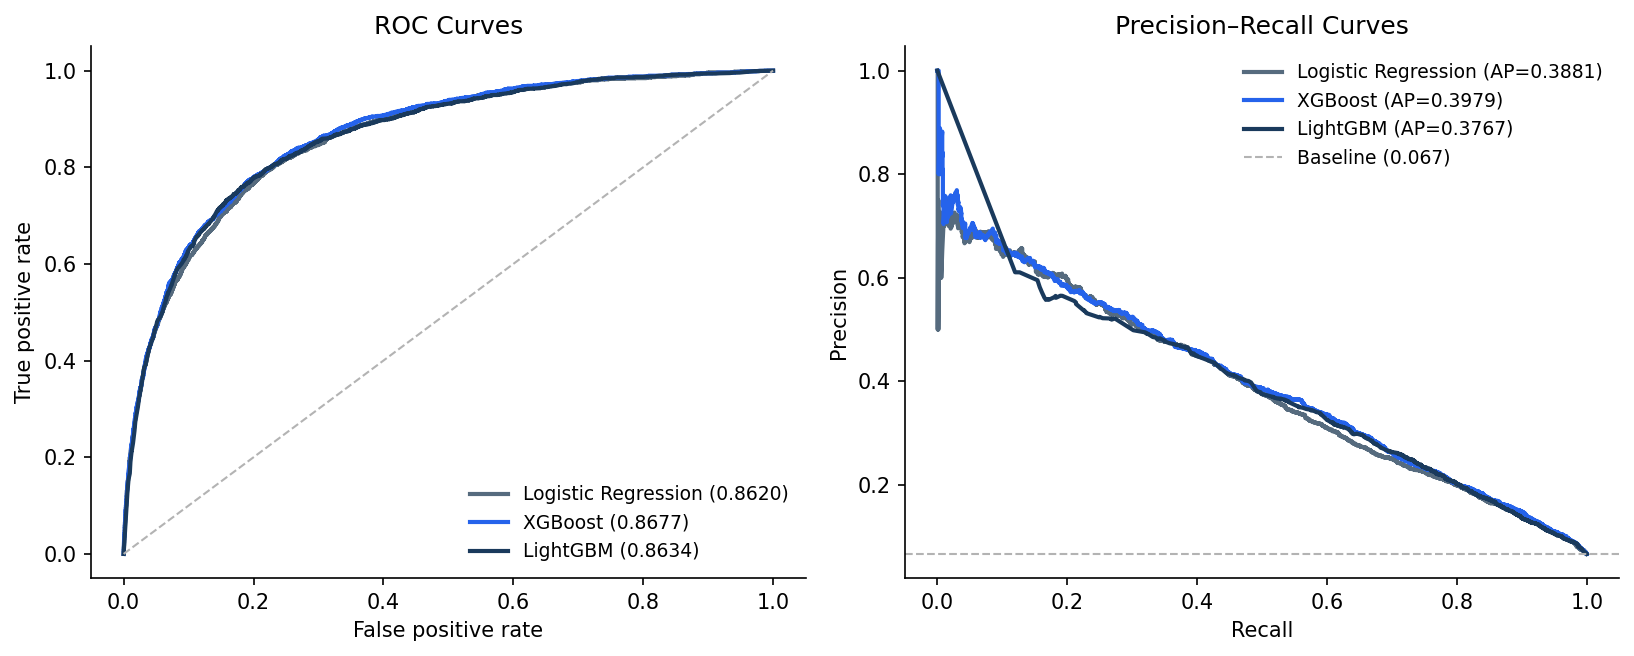
\includegraphics[width=0.92\textwidth]{fig_roc_pr.png}
\caption{ROC (left) and precision--recall (right) curves on the holdout set.
All three models occupy nearly the same ROC space, though XGBoost leads
narrowly. The precision--recall curves diverge more at high recall,
highlighting the effect of class imbalance.}
\label{fig:roc}
\end{figure}

\subsection{SHAP Feature Importance}

The global SHAP analysis (Figure~\ref{fig:shap_bar} and Figure~\ref{fig:shap_bee})
reveals a clear two-tier structure. \texttt{RevolvingUtilizationOfUnsecuredLines}
dominates with a mean absolute SHAP of 0.198 --- nearly 1.5 times larger than
the second feature, \texttt{MaxDelqStatus} (0.131). Together they account for
roughly two thirds of the total feature impact signal. Age comes third at 0.043,
followed by monthly income (0.030) and estimated monthly debt burden (0.028).
The bottom half of the feature ranking contributes comparatively little.

\begin{figure}[h]
\centering
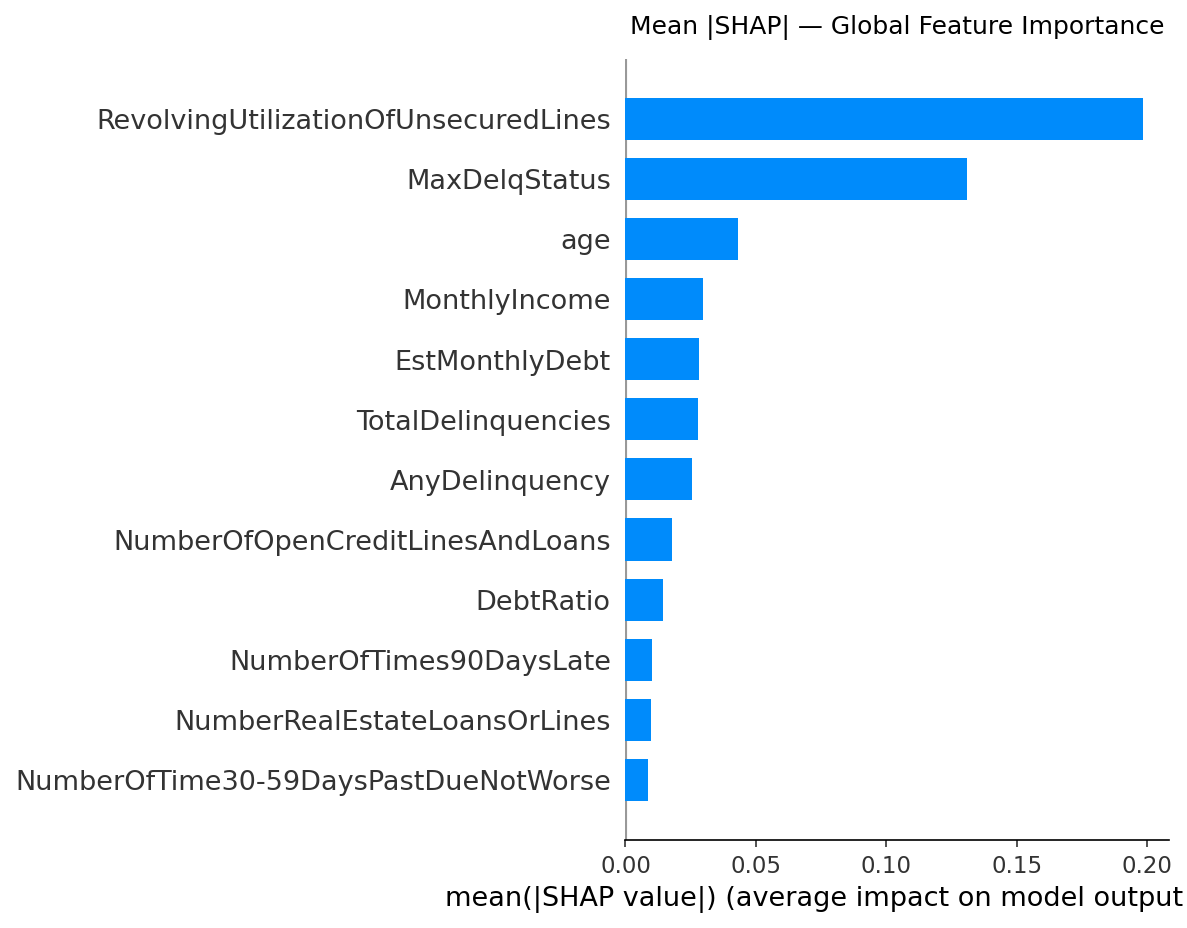
\includegraphics[width=0.80\textwidth]{fig_shap_bar.png}
\caption{Global feature importance measured by mean absolute SHAP value.
Revolving credit utilisation and maximum delinquency status together dominate,
consistent with credit bureau practice.}
\label{fig:shap_bar}
\end{figure}

\begin{figure}[h]
\centering
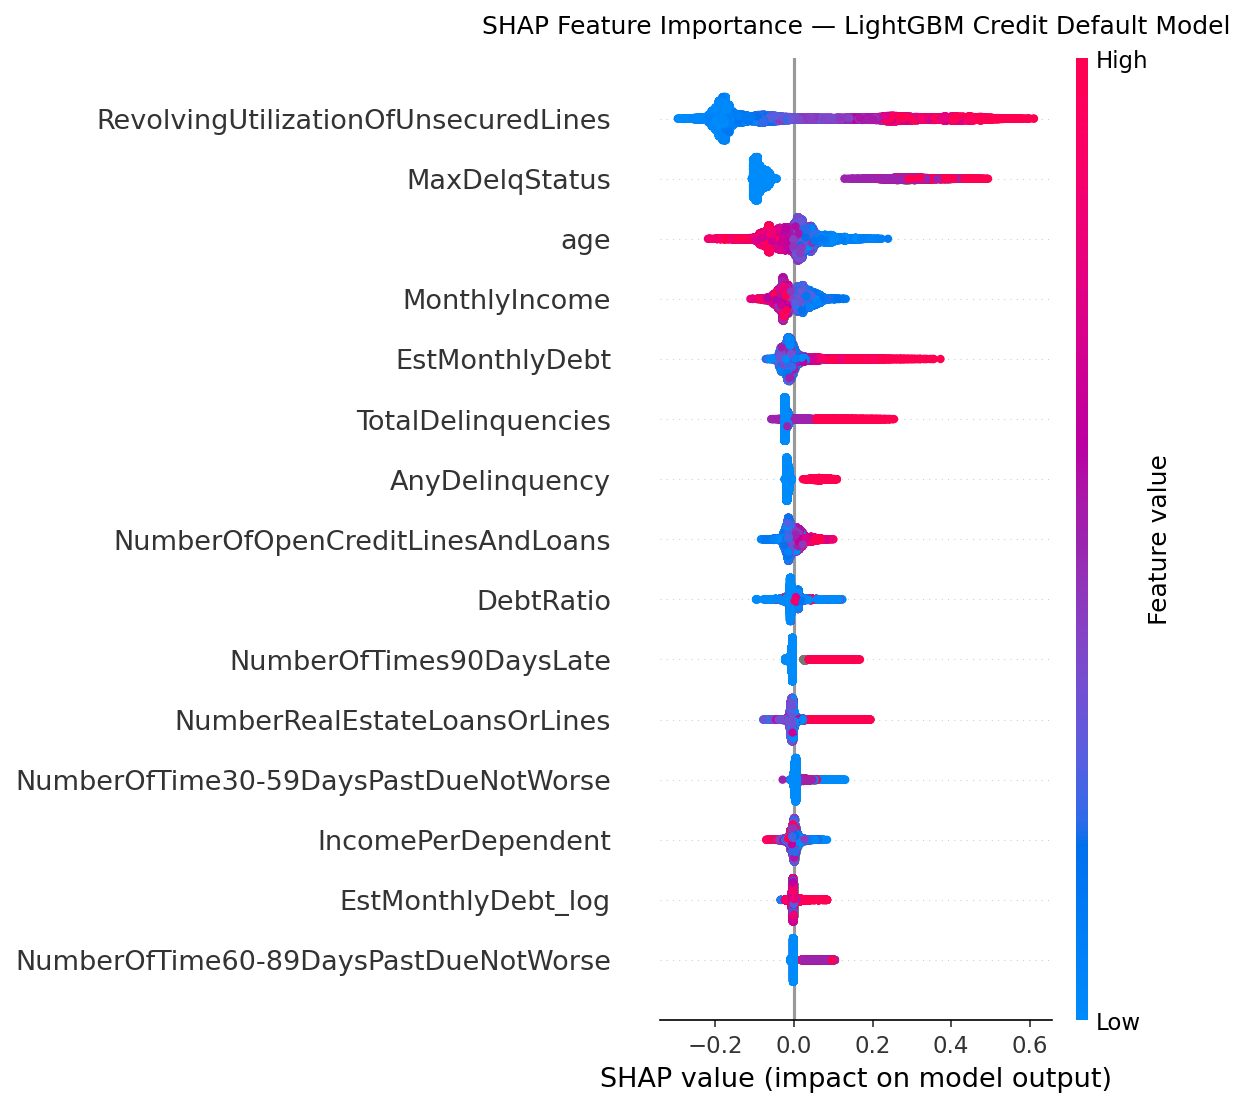
\includegraphics[width=0.80\textwidth]{fig_shap_beeswarm.png}
\caption{SHAP beeswarm plot. Each dot is one borrower from the holdout set.
Colour indicates feature value (red\,=\,high, blue\,=\,low); horizontal position
shows the direction and magnitude of impact on the predicted default probability.
High revolving utilisation and any history of delinquency consistently push
predictions towards default.}
\label{fig:shap_bee}
\end{figure}

The beeswarm plot tells a coherent story that any credit officer would
recognise. Borrowers who have already pushed their revolving credit lines
close to the limit are signalling financial stress that predates an actual
missed payment --- the model picks this up clearly, with SHAP values
reaching as high as 0.61 for fully-utilised lines. For delinquency history,
the effect is similarly intuitive: even a single prior late payment
(MaxDelqStatus\,=\,1) shifts the predicted probability meaningfully upward.
Age runs in the opposite direction --- younger borrowers carry higher
predicted risk, older borrowers lower, consistent with the empirical
regularity that default rates peak in the 20s and 30s and decline with
credit age~\cite{siddiqi2012credit}.

\subsection{SHAP Dependence Plots}

Figure~\ref{fig:shap_dep} examines the three dominant features in detail.
For revolving utilisation, the relationship is roughly monotone but
non-linear: the SHAP value increases gradually up to around 0.5 utilisation
and then accelerates sharply, suggesting a threshold effect. This aligns with
industry rules of thumb that flag utilisation above 30--50\,\% as a
risk signal. The interaction colour (AnyDelinquency) shows that borrowers
with prior delinquencies (red) receive even larger SHAP penalties at high
utilisation levels --- the two risks compound.

For MaxDelqStatus, the jump from zero to one is the largest single step,
after which additional delinquency severity adds incrementally. This makes
sense: the key distinction is between borrowers who have never missed a
payment and those who have, not between mild and severe delinquency.
For age, the effect is most pronounced below 40, after which the
protective effect of age plateaus.

\begin{figure}[h]
\centering
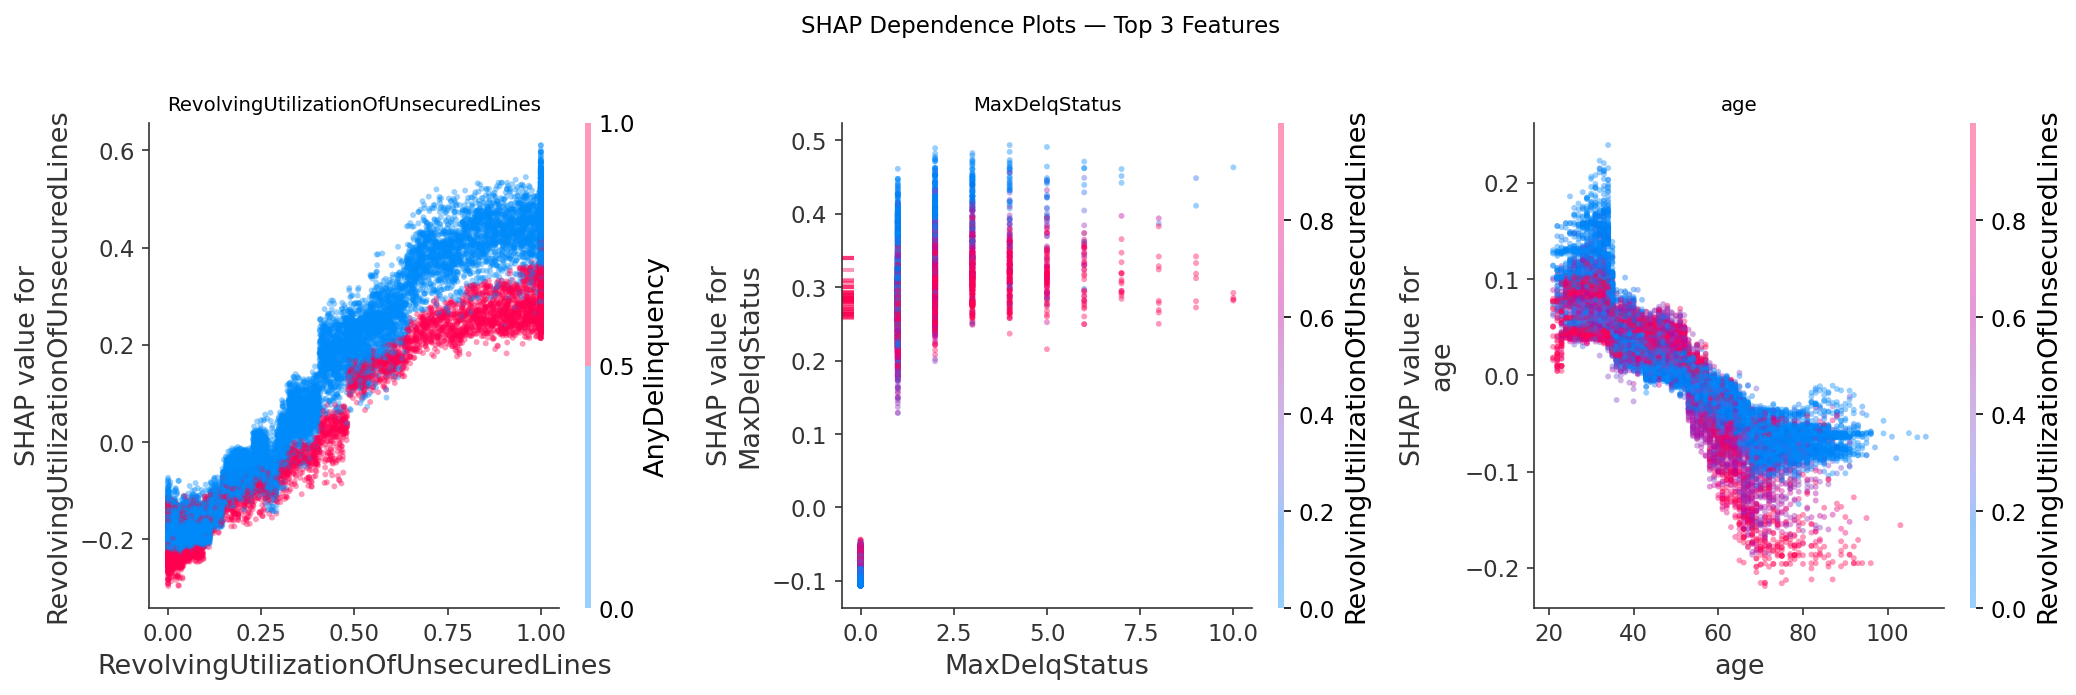
\includegraphics[width=\textwidth]{fig_shap_dependence.png}
\caption{SHAP dependence plots for the three most important features.
Left: revolving utilisation shows a non-linear threshold effect around 0.5,
amplified for borrowers with prior delinquency (interaction colour).
Centre: the MaxDelqStatus jump from 0 to 1 carries the largest risk increment.
Right: age is protective, with the effect strongest for borrowers under 40.}
\label{fig:shap_dep}
\end{figure}

\subsection{Model Calibration}

Figure~\ref{fig:calib} reveals a limitation that the AUROC numbers hide:
none of the three models produces well-calibrated probabilities. The tree
models in particular show erratic calibration curves, with LightGBM
exhibiting a pronounced spike at intermediate predicted probabilities.
This matters for microfinance applications where the model's output might
be used to set a risk threshold (e.g., ``decline applications with
predicted default probability above 15\,\%''). If the predicted probability
does not correspond to an actual default rate, that threshold has no
reliable interpretation.

\begin{figure}[h]
\centering
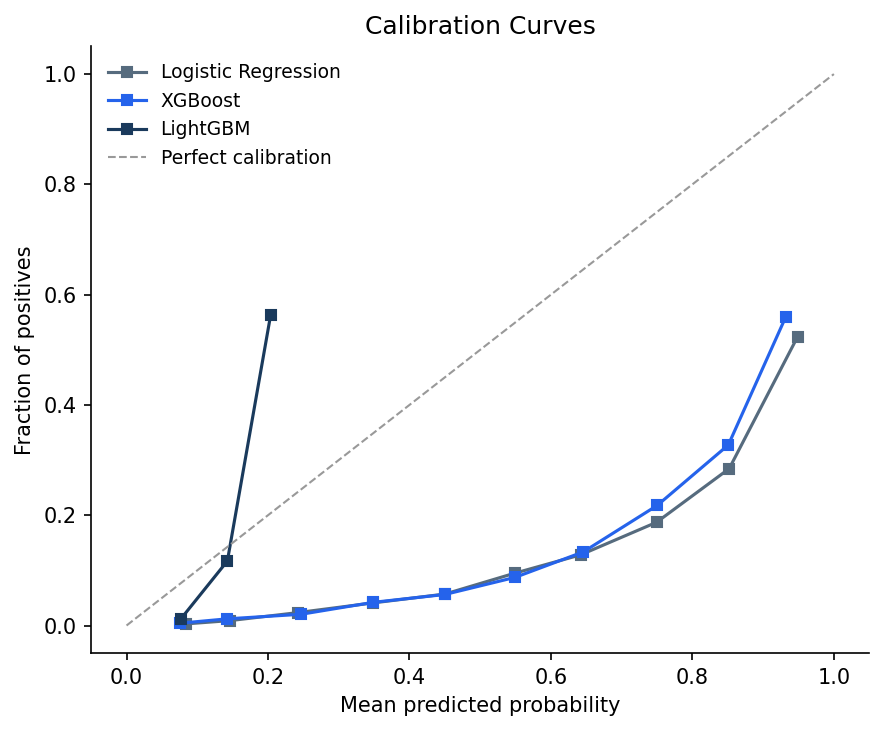
\includegraphics[width=0.62\textwidth]{fig_calibration.png}
\caption{Calibration curves for all three models. A perfectly calibrated
model would follow the dashed diagonal. All three models deviate substantially,
suggesting that Platt scaling or isotonic regression should be applied before
probabilities are used as decision thresholds.}
\label{fig:calib}
\end{figure}

Post-hoc calibration via Platt scaling~\cite{platt1999probabilistic} or
isotonic regression is therefore recommended before deploying these models
in a production lending system.

\section{Discussion}

The results paint a consistent picture. Gradient boosting is the better
classifier on this dataset, but not dramatically so --- Logistic Regression
gets surprisingly close, which suggests that the features themselves carry
most of the signal and the model choice matters less than it might seem.
For a microfinance lender who needs a regulator-approved, auditable model,
that is actually good news: there is not much to lose by choosing the
simpler option.

The SHAP analysis adds something that the metrics alone cannot: a credible
account of what the model has actually learned. The fact that revolving
utilisation and delinquency history dominate, while income and debt ratio
play a supporting role, matches what credit practitioners have known for
decades. When a model's learned representation agrees with domain knowledge,
that is evidence it is generalising rather than memorising. It also makes
the model easier to defend to regulators: we can point to specific,
interpretable features and explain why each one is included.

The calibration finding is perhaps the most practically important result in
the paper. It is easy to treat a model's output as a probability estimate
and set approval thresholds accordingly. The calibration curves show this
would be a mistake without recalibration. We flag this as a required
post-processing step for any real deployment.

For microfinance lenders in East Africa, two additional caveats are worth
stating. First, this dataset reflects US consumer credit behaviour; the
feature distributions, default rates, and feature interactions may look
different for mobile credit customers in Kenya or Uganda. Transfer without
local validation would be inadvisable. Second, 19.8\,\% of borrowers
are missing income data; any production system needs a principled missing
data strategy rather than simple median imputation.

\section{Limitations}

This study uses a single dataset from one country and one time period. The
models are validated on a random holdout rather than a temporal split, which
overstates real-world performance because it does not account for
distributional drift over time. Hyperparameters were tuned informally
rather than via systematic cross-validation. The SHAP analysis is computed
on LightGBM only; XGBoost SHAP values may differ slightly given the small
performance gap between the two models. Finally, we do not evaluate the
models for fairness (disparate impact across demographic groups); given the
regulatory environment for credit, this is a meaningful omission that future
work should address.

\section{Conclusion}

We trained and compared three classifiers on a consumer credit default
dataset and used SHAP to open up the best-performing model's decision
logic. The headline result is that revolving credit utilisation and
prior delinquency history together account for the dominant share of
predictive signal, a finding that aligns cleanly with established credit
theory and supports the model's face validity. All three classifiers are
competitive, which suggests that lenders who prioritise interpretability
can choose Logistic Regression without paying much in predictive accuracy.
The calibration analysis highlights a gap between ranking performance
(measured by AUROC) and probability reliability that has direct
implications for threshold-based lending decisions. Together, these
findings make a case for SHAP-augmented gradient boosting as a
practical, explainable credit scoring framework for microfinance lenders
operating under regulatory transparency requirements.

\section*{Reproducibility}
The full training code, notebook, and saved model are publicly available
at \url{https://github.com/craigouma}.

\begin{thebibliography}{9}

\bibitem{lundberg2017shap}
S.~M.~Lundberg and S.-I.~Lee,
``A unified approach to interpreting model predictions,''
in \emph{Advances in Neural Information Processing Systems (NeurIPS)},
vol.~30, 2017.

\bibitem{chen2016xgboost}
T.~Chen and C.~Guestrin,
``XGBoost: A scalable tree boosting system,''
in \emph{Proceedings of the 22nd ACM SIGKDD International Conference on
Knowledge Discovery and Data Mining}, pp.~785--794, 2016.

\bibitem{ke2017lightgbm}
G.~Ke, Q.~Meng, T.~Finley, T.~Wang, W.~Chen, W.~Ma, Q.~Ye, and T.-Y.~Liu,
``LightGBM: A highly efficient gradient boosting decision tree,''
in \emph{Advances in Neural Information Processing Systems (NeurIPS)},
vol.~30, 2017.

\bibitem{lessmann2015benchmarking}
S.~Lessmann, B.~Baesens, H.-V.~Seow, and L.~C.~Thomas,
``Benchmarking state-of-the-art classification algorithms for credit scoring:
An update of research,''
\emph{European Journal of Operational Research}, vol.~247, no.~1,
pp.~124--136, 2015.

\bibitem{bussmann2021explainability}
N.~Bussmann, P.~Giudici, D.~Marinelli, and J.~Papenbrock,
``Explainability for fair machine learning in credit scoring,''
\emph{Journal of Financial Data Science}, vol.~3, no.~1,
pp.~26--43, 2021.

\bibitem{siddiqi2012credit}
N.~Siddiqi,
\emph{Credit Risk Scorecards: Developing and Implementing Intelligent
Credit Scoring}.
Wiley, 2nd ed., 2012.

\bibitem{barocas2023fairness}
S.~Barocas, M.~Hardt, and A.~Moritz,
\emph{Fairness and Machine Learning: Limitations and Opportunities}.
MIT Press, 2023.

\bibitem{platt1999probabilistic}
J.~Platt,
``Probabilistic outputs for support vector machines and comparisons to
regularized likelihood methods,''
\emph{Advances in Large Margin Classifiers}, vol.~10, no.~3,
pp.~61--74, 1999.

\bibitem{demirguc2018financial}
A.~Demirguc-Kunt, L.~Klapper, D.~Singer, S.~Ansar, and J.~Hess,
\emph{The Global Findex Database 2017: Measuring Financial Inclusion and
the Fintech Revolution}.
World Bank, 2018.

\end{thebibliography}

\end{document}
